\documentclass[10pt,a4paper]{article}
\usepackage[margin=21mm]{geometry}
\usepackage{fontspec}
\setmainfont{lmroman10-regular.otf}[BoldFont=lmroman10-bold.otf,ItalicFont=lmroman10-italic.otf,BoldItalicFont=lmroman10-bolditalic.otf]
\usepackage{amsmath,amssymb,booktabs,tabularx,array,graphicx,caption,fancyhdr,xcolor}
\usepackage[authoryear,round]{natbib}
\usepackage[unicode,colorlinks=true,linkcolor=black,citecolor=black,urlcolor=blue]{hyperref}
\usepackage{xurl,microtype}
\DeclareMathSizes{10}{10}{7}{7}
\setlength{\parindent}{0pt}\setlength{\parskip}{4pt}
\setlength{\emergencystretch}{3em}
\renewcommand{\arraystretch}{1.08}
\captionsetup{font=footnotesize,labelfont=bf}
\setcounter{topnumber}{4}\renewcommand{\topfraction}{.95}\renewcommand{\textfraction}{.06}\renewcommand{\floatpagefraction}{.75}
\setlength{\textfloatsep}{10pt}\setlength{\intextsep}{10pt}
\pagestyle{fancy}\fancyhf{}\fancyhead[L]{\small Hakan Zeki Gülmez}\fancyhead[R]{\small SBA 7(a) lending}\fancyfoot[C]{\thepage}\setlength{\headheight}{13pt}
\definecolor{blue}{HTML}{0072B2}
\newcommand{\losslabel}{EAD = GrossApproval; full-disbursement proxy, CCF = 100\%. LGD is the gross charge-off proxy on the same approval denominator. SBA/lender amounts use assumption-based pro-rata guarantee allocation.}
\newcommand{\scenario}{Scenario projections on the fixed 2006 portfolio; not out-of-sample validation.}
\newcommand{\tbl}[2]{\begin{table}[htbp]\centering\input{generated/#1.tex}\caption{#2}\end{table}}
\newcommand{\datafile}[1]{\href{https://github.com/hakangulmez/credit-risk-sba}{\nolinkurl{#1}}}
\input{generated/numbers.tex}

\begin{document}
\begin{center}
{\LARGE\bfseries Local economic conditions and public--lender loss sharing in SBA 7(a) lending}\par
\vspace{5pt}Hakan Zeki Gülmez\par
\small M.Sc. Management \& Technology (Economics \& Econometrics), Technical University of Munich\par October 2026 • Local review draft
\end{center}
\textbf{Question.} How do recorded charge-off risk and assumption-based loss sharing vary across cohorts and fixed economic scenarios in approved and disbursed SBA lending?

\textbf{Data and method.} We use the official SBA FOIA snapshot of 30 June 2026, including unresolved status records with complete follow-up; the outcome is recorded charge-off within 36 months of first disbursement, not observed delinquency. We estimate Term-free Firth logistic models: Layer 1 reconstructs approval descriptors, while Layer 2 conditions on future realized or stipulated BLS unemployment and FHFA house-price paths. We compare saved out-of-time metrics, calibration groups and fixed-portfolio scenarios; the two uncertainty procedures condition on different fixed inputs.

\begin{figure}[h!]\centering
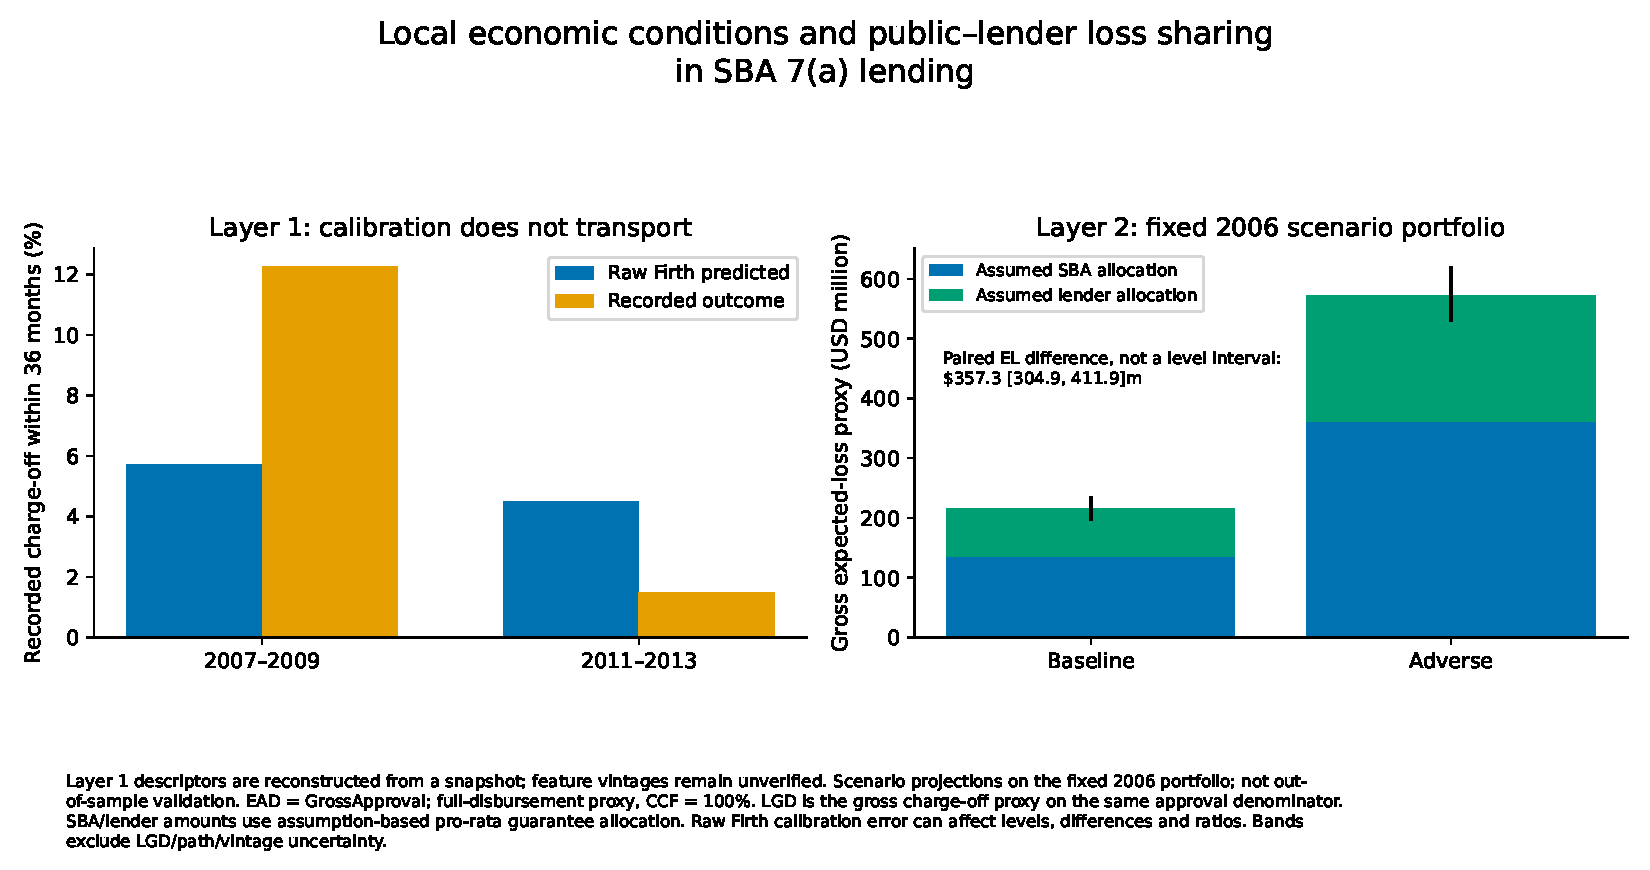
\includegraphics[width=\linewidth]{../../figures/g5/headline.pdf}
\caption{Raw Firth evidence across different information sets. Left: Layer 1 evaluation cohorts. Right: \scenario\ \losslabel\ Marginal total-loss bands are distinct from the labelled paired-difference interval. Calibration error can affect levels, differences and ratios.}
\end{figure}
\textbf{Finding 1 — Ranking survives modestly; calibration fails.} Crisis AUC is \AucCrisis, compared with \AucLater\ in the later cohort. Predicted/recorded rates are \PdCrisis\%/\RateCrisis\% and \PdLater\%/\RateLater\%, respectively. These results do not establish stable transportability; causes of the cohort differences are not identified.

\textbf{Source notice.} Official SBA 7(a) FOIA; direct BLS LAUS and FHFA all-transactions state HPI. This product uses FHFA data but is neither endorsed nor certified by FHFA. No FRED observations or borrower-level data are distributed. Full source hashes, selectors and interval provenance are in CLAIMS.md and the technical report.
\newpage
\section*{Conditional associations and loss sharing}
\textbf{Finding 2 — The path definition matters.} Define endpoint $\Delta u=u_{36}-u_0$ and peak $\max_{m=0,\ldots,36}(u_m-u_0)$. On the fixed observed portfolio, a conditional +1 percentage point change in endpoint unemployment gives \Endpoint\ probability percentage points; the separately estimated peak-path sensitivity gives \Peak. These are finite-change associations, not derivatives or causal effects. The peak specification addresses increases that subsequently reverse, without replacing the primary specification.

\textbf{Finding 3 — Allocation depends on assumptions and scenario weights.} Baseline/adverse EL proxies are \ElBase\ and \ElAdverse\ million dollars, an arithmetic ratio of \ElRatio. The paired adverse-minus-baseline difference is \ElDiff\ million dollars. Assumed SBA shares are \ShareBase\% and \ShareAdverse\%; different scenario PDs reweight loans, so aggregate shares need not be constant. The split measures neither observed guarantee payments nor fiscal costs or lender behaviour. \scenario

\textbf{A separate Layer 2 calibration check.} In the retrospective 2013--2014 cohort, raw Firth predicts \LtwoFirth\% against \LtwoRate\% recorded. Calibrated LightGBM predicts \LtwoTree\%, close to the same average, but its intercept is \TreeIntercept\ and slope \TreeSlope; their stored intervals exclude ideal values. Training-score groups retain miscalibration. Average agreement does not solve calibration.

\textbf{Chronology and inference.} Layer 1 estimates on 1991--2002. Benchmark settings selected on 2003H1 in G2 are inherited unchanged; benchmark calibration uses 2003H2. Layer 2 estimates on 1991--2009 and calibrates LightGBM only on 2010. Its check uses future realized macro paths, its calibration labels overlap the 2013 calendar, and the 2013 cohort was already inspected. The scenario portfolio is included in Layer 2 estimation. Stored fitted-model evaluation bands differ from training-state multiplier refit intervals, which hold preprocessing, portfolio, LGD and paths fixed; they exclude calibration-model, scenario-construction and source-vintage uncertainty.

\colorbox{blue!6}{\parbox{.965\linewidth}{\textbf{Limitations}\begin{itemize}\setlength\itemsep{2pt}
\item Administrative charge-off and unresolved EXEMPT status do not establish delinquency or performance; rejected applicants are outside the sample.
\item Descriptor and Term vintages remain unverified; the Term audit verdict is ``Timing unverifiable.'' Primary models stay Term-free. Rates are largely missing.
\item Revised macro vintages, future-path conditioning, reused cohorts and a post-results amendment preclude a real-time or untouched-confirmatory claim.
\item \losslabel\ Recovery, amortization and actual payouts are unobserved. Full utilization does not establish that combined EL is necessarily conservative.
\item Independent-state and successful-draw assumptions constrain intervals. State-specific adverse flags affect \SupportShare\% of loans; univariate checks do not establish joint support or path plausibility.
\end{itemize}}}

\small No new fitting, prediction, recalibration or empirical analysis was performed for this write-up. External release requires separate approval. Results and complete qualifications: technical report and CLAIMS.md; local drafts only.
\end{document}
